\documentclass[]{article}
\usepackage{amsmath}
\usepackage{amsfonts}
\usepackage{amssymb}
\usepackage{amsthm}
\usepackage{cancel}
\usepackage{graphicx}
\usepackage{siunitx}
\usepackage{circuitikz}
\usepackage{pdfpages}
\usepackage{hyperref}

\renewcommand{\thesection}{\arabic{section}}
\renewcommand{\thesubsection}{\thesection.\alph{subsection}}
\renewcommand{\thesubsubsection}{\thesubsection.\roman{subsubsection}}

\newtheorem{genthm}{Theorem}

%opening
\title{EECS 16A HW11}
\author{Bryan Ngo}
\date{2019-11-13}

\begin{document}

\maketitle

\section{MP3 Player}

\subsection{}

\begin{center}
\begin{circuitikz}[american]
	\draw (0, 2) to[V_=\(V_{ref}\)] (0, 0) node[ground]{};
	\draw (0, 2) to[short] (3, 2);
	\draw (3, 2) to[C=\(C_1\), v=\(V_1\)] (3, 0) node[ground]{};
\end{circuitikz}
\end{center}

\subsection{}

\begin{center}
\begin{circuitikz}[american]
	\draw (0, 2) to[C=\(C_1\), v=\(V_1\)] (0, 0) node[ground]{};
	\draw (0, 2) to[short] (3, 2);
	\draw (3, 2) to[C=\(C_2\), v=\(V_2\)] (3, 0) node[ground]{};
\end{circuitikz}
\end{center}

\subsection{}

\begin{center}
\begin{tabular}{||l|l|l|l||}
	\hline
	\textbf{Step} & \(b\) & \(V_{n1}\) & \(V_{n2}\) \\
	\hline
	1 & 0 & \SI{0}{\volt} & \SI{0}{\volt} \\
	2 & 1 & \(V_{\text{ref}}\) & \(V_{\text{ref}} / 2\) \\
	3 & 0 & \SI{0}{\volt} & \(V_{\text{ref}} / 4\) \\
	4 & 1 & \(V_{\text{ref}}\) &  \(5 V_{\text{ref}} / 8\) \\
	\hline
\end{tabular}
\end{center}

During Step 3 phase 1, since \(b = 0\), \(S_1\) is open, \(S_2\) is closed, \(S_3\) is open, shorting \(C_1\) to \SI{0}{\volt}. 
Then during phase 2, \(S_3\) closes and the voltage across the caps is the same. 
Since they are at the same capacitance, the voltage across both is simply the average of the two individual voltages. \\
\\
During Step 4 phase 1, \(C_1\) is brought to \(V_{\text{ref}}\) and \(C_2\) remains at \(V_{\text{ref}} / 4\). 
During phase 2, they share, so we average the voltages once more. 

\subsection{}

Note the \(V_{n2}\) is the average of the two individual voltages, and \(V_{n1}\) is either \SI{0}{\volt} or \(V_{\text{ref}}\). 
From this, we can find that the phase 2 \(V_{n2}\) was previously
\begin{equation}
	V_{prev} = 2 V_{n2} - V_{\text{ref}} = \frac{5 V_{\text{ref}}}{8}
\end{equation}
Note that this is the same voltage as step 4 for problem 1.c. 
This means that the control sequence must be \(b = \{1, 0, 1, 1\}\) since we can move everything up one step by immediately charging the capacitors and then leaving \(C_1\) at \(V_{\text{ref}}\) during phase 1 of step 4. 

\section{Integration using Op-amps}

\subsection{}

Applying KCL to the negative terminal of the op-amp, 
\begin{align}
	I_{R_1} - i_{C_1} - \cancel{I^-} &= 0 \\
	\frac{v_0 - \cancel{V^-}}{R_1} - C_1 \frac{d V_{C_1}}{dt} &= 0 \\
	\frac{d V_{C_1}}{dt} &= \frac{v_0}{R_1 C_1} \\
	V_{C_1} &= \frac{v_0}{R_1 C_1} t
\end{align}
Here \(I^-, V^-\) are nulled because of the golden rules of op-amps. 
Since the negative terminal of the capacitor is facing the positive terminal of \(v_1\), 
\begin{equation}
	v_1 = -V_{C_1} = -\frac{v_0}{R_1 C_1} t
\end{equation}
with a slope of \(-\frac{v_0}{R_1 C_1}\). 

\subsection{}

Going back to the first KCL equation, we found that 
\begin{equation}
	i_{C_1} = I_{R_1} = \frac{v_0}{R_1}
\end{equation}
Note that this is independent of \(C_1\), so the current should not change regardless of the capacitance. 
However, if we were to double the capacitance, the ramp slope should decrease, since \(v_1 \propto \frac{1}{C_1}\). 

\subsection{}

Adding a load resistance to \(v_1\) should not change the actual value of \(v_1\) since \(v_1\) is only dependent on components that do not change with the addition of a new load. 

\subsection{}

\begin{center}
	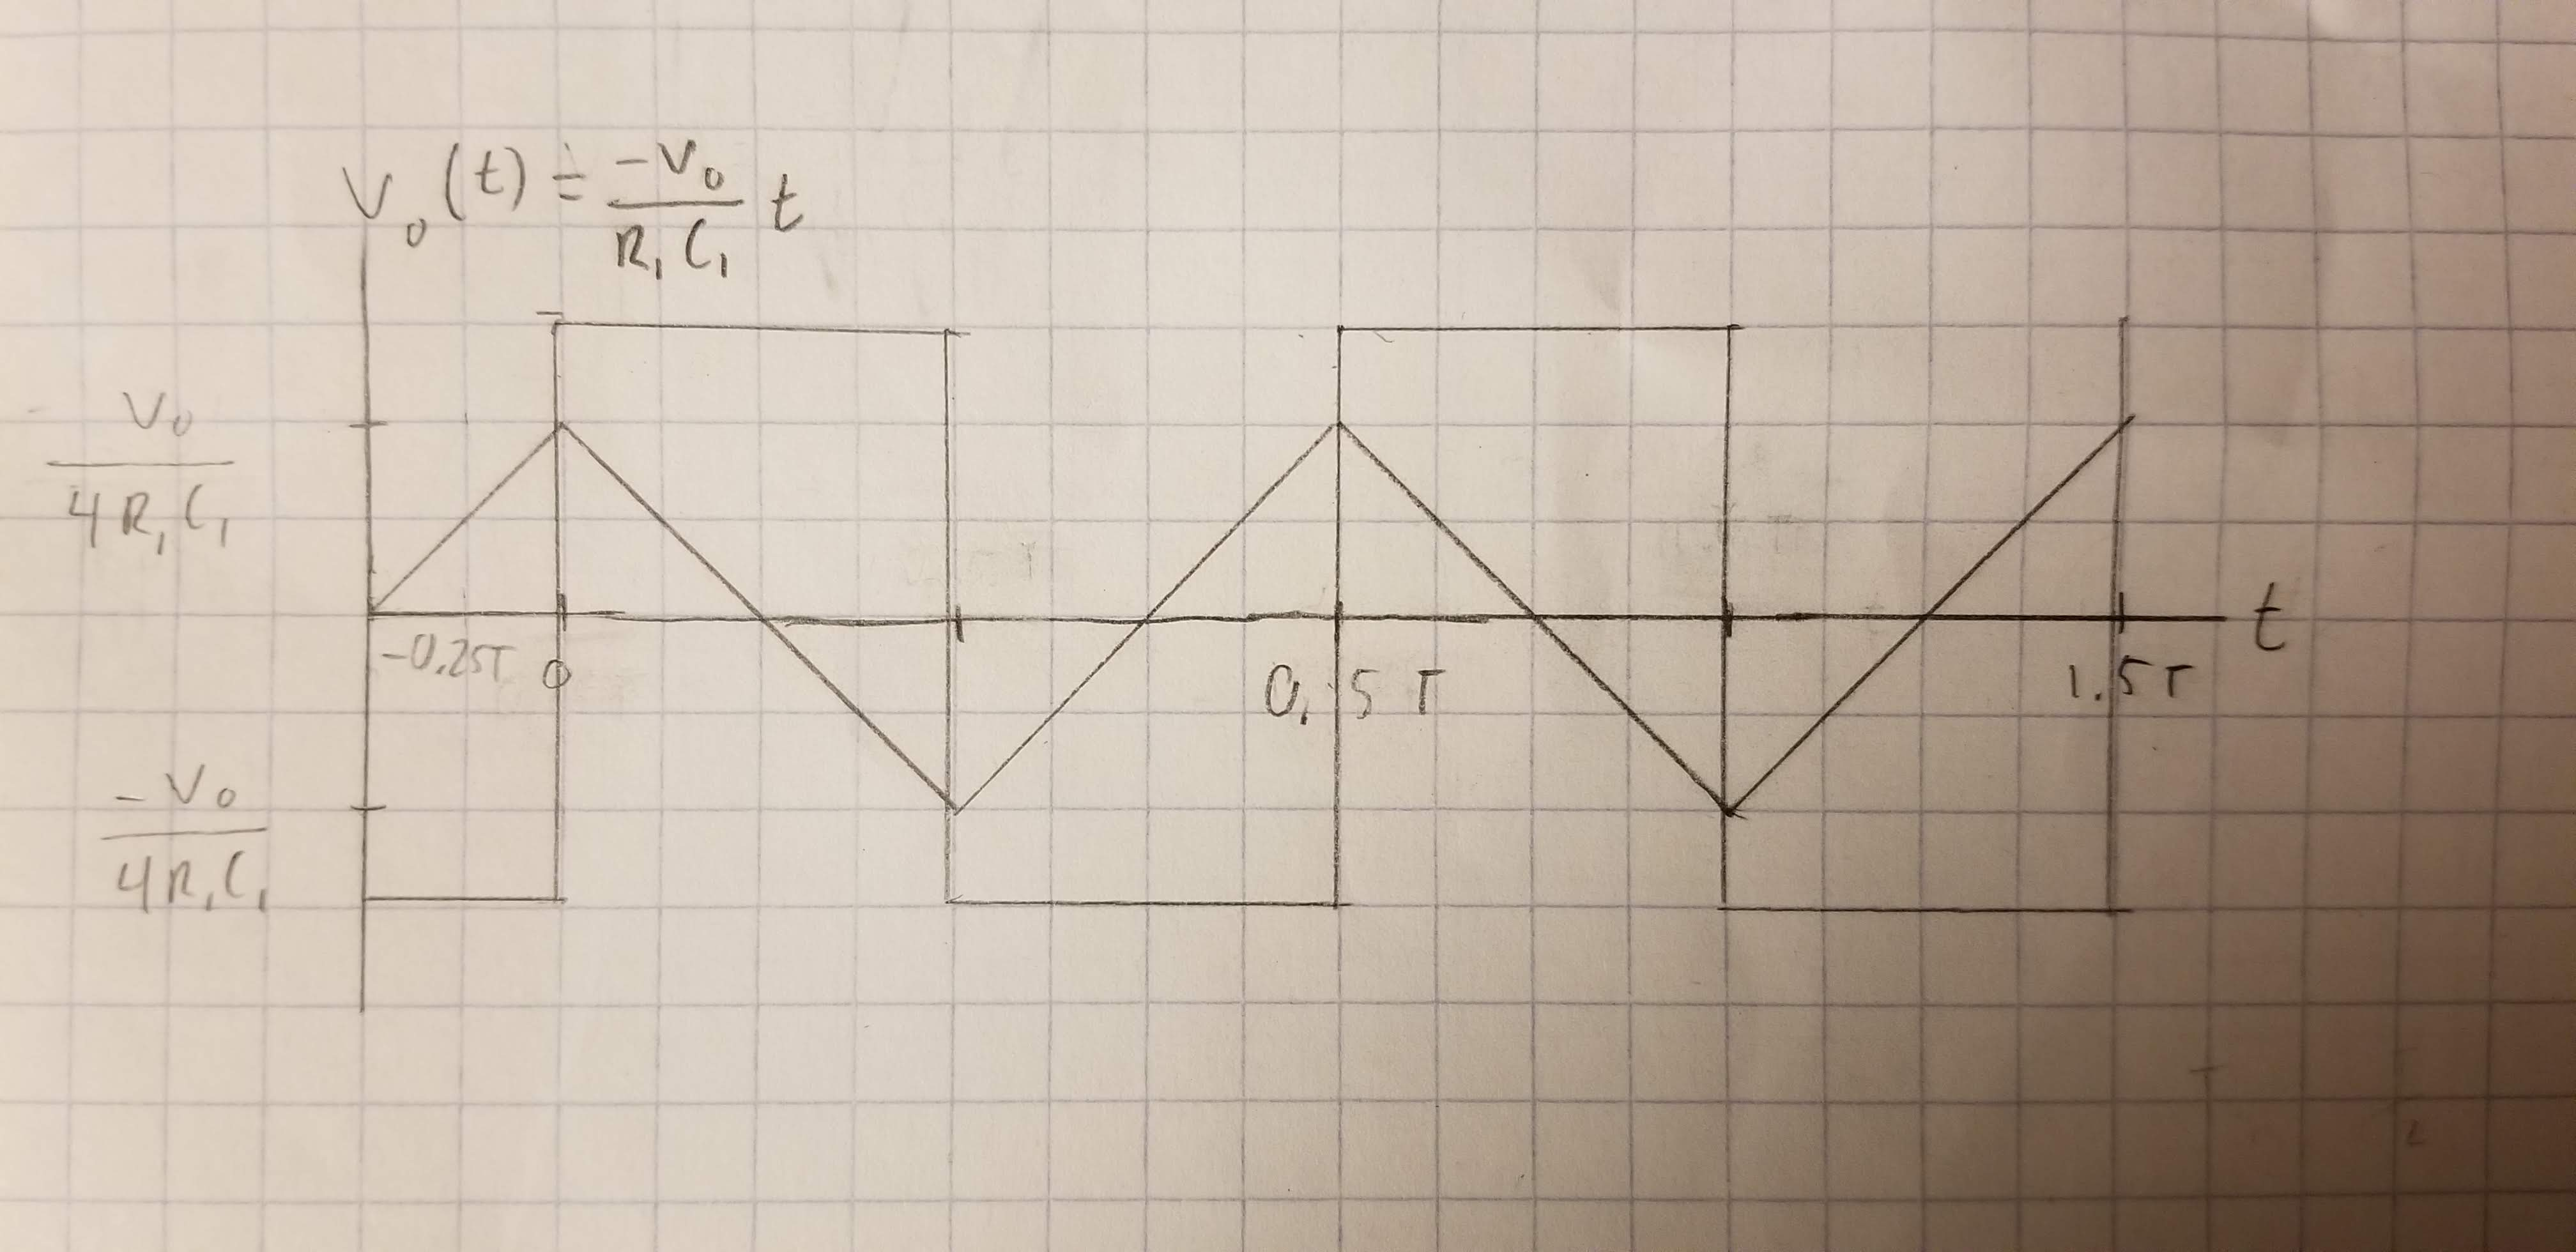
\includegraphics[width=0.7\linewidth]{20191115_195045}
\end{center}

\subsection{}

\begin{equation}
	R \cdot C = \frac{\si{\volt}}{\si{\ampere}} \cdot \frac{\si{\coulomb}}{\si{\volt}} = \frac{\si{\coulomb}}{\si{\coulomb\per\second}} = \frac{1}{\si{\per\second}} = \si{\second}
\end{equation}

\section{Cool for the Summer}

\subsection{}

Using the golden rules of op-amps, the KCL for the negative terminal is 
\begin{align}
	I_{R_1} - I_{R_2} - \cancel{I^-} &= 0 \\
	\frac{v_{in} - \cancel{V^-}}{R_1} &= \frac{-u}{R_2}
\end{align}
where \(u\) is the node at the output terminal. 
Substituting \(v_{out} = u\), 
\begin{equation}
	v_{out} = -v_{in}\frac{R_2}{R_1}
\end{equation}

\subsection{}

The KCL equation is 
\begin{align}
	\frac{v_{s1}}{R_{s1}} + \frac{v_{s2}}{R_{s2}} &= \frac{-u}{R_2} \\
	v_{out} &= -R_2 \left(\frac{v_{s1}}{R_{s1}} + \frac{v_{s2}}{R_{s2}}\right)
\end{align}

\subsection{}
We pick \(R_{s1} = \SI{4}{\ohm}\), \(R_{s2} = \SI{0.5}{\ohm}\), \(R_{2} = \SI{1}{\ohm}\). 

\subsection{}

\begin{center}
\begin{circuitikz}[american]
	\draw (1, 0) node[op amp](opamp){}
	(opamp.+) node[ground]{};
	\draw (-4, 0.5) to[R=\SI{1}{\ohm}, o-] (0, 0.5) to[short] (opamp.-);
	\draw (opamp.-) to[short] (-0.2, 2) to[R=\SI{1}{\ohm}] (2.2, 2) to[short] (opamp.out);
	\draw (opamp.out) to[short] (4, 0) node[ocirc]{\, \(-v_{out}\)};
	\draw (-4, 0.5) to[open, v=\(v_{out}\)] (-4, -0.5) node[ground]{};
\end{circuitikz}
\end{center}

\section{Petbot Design}

\subsection{Speed Control}

\begin{center}
	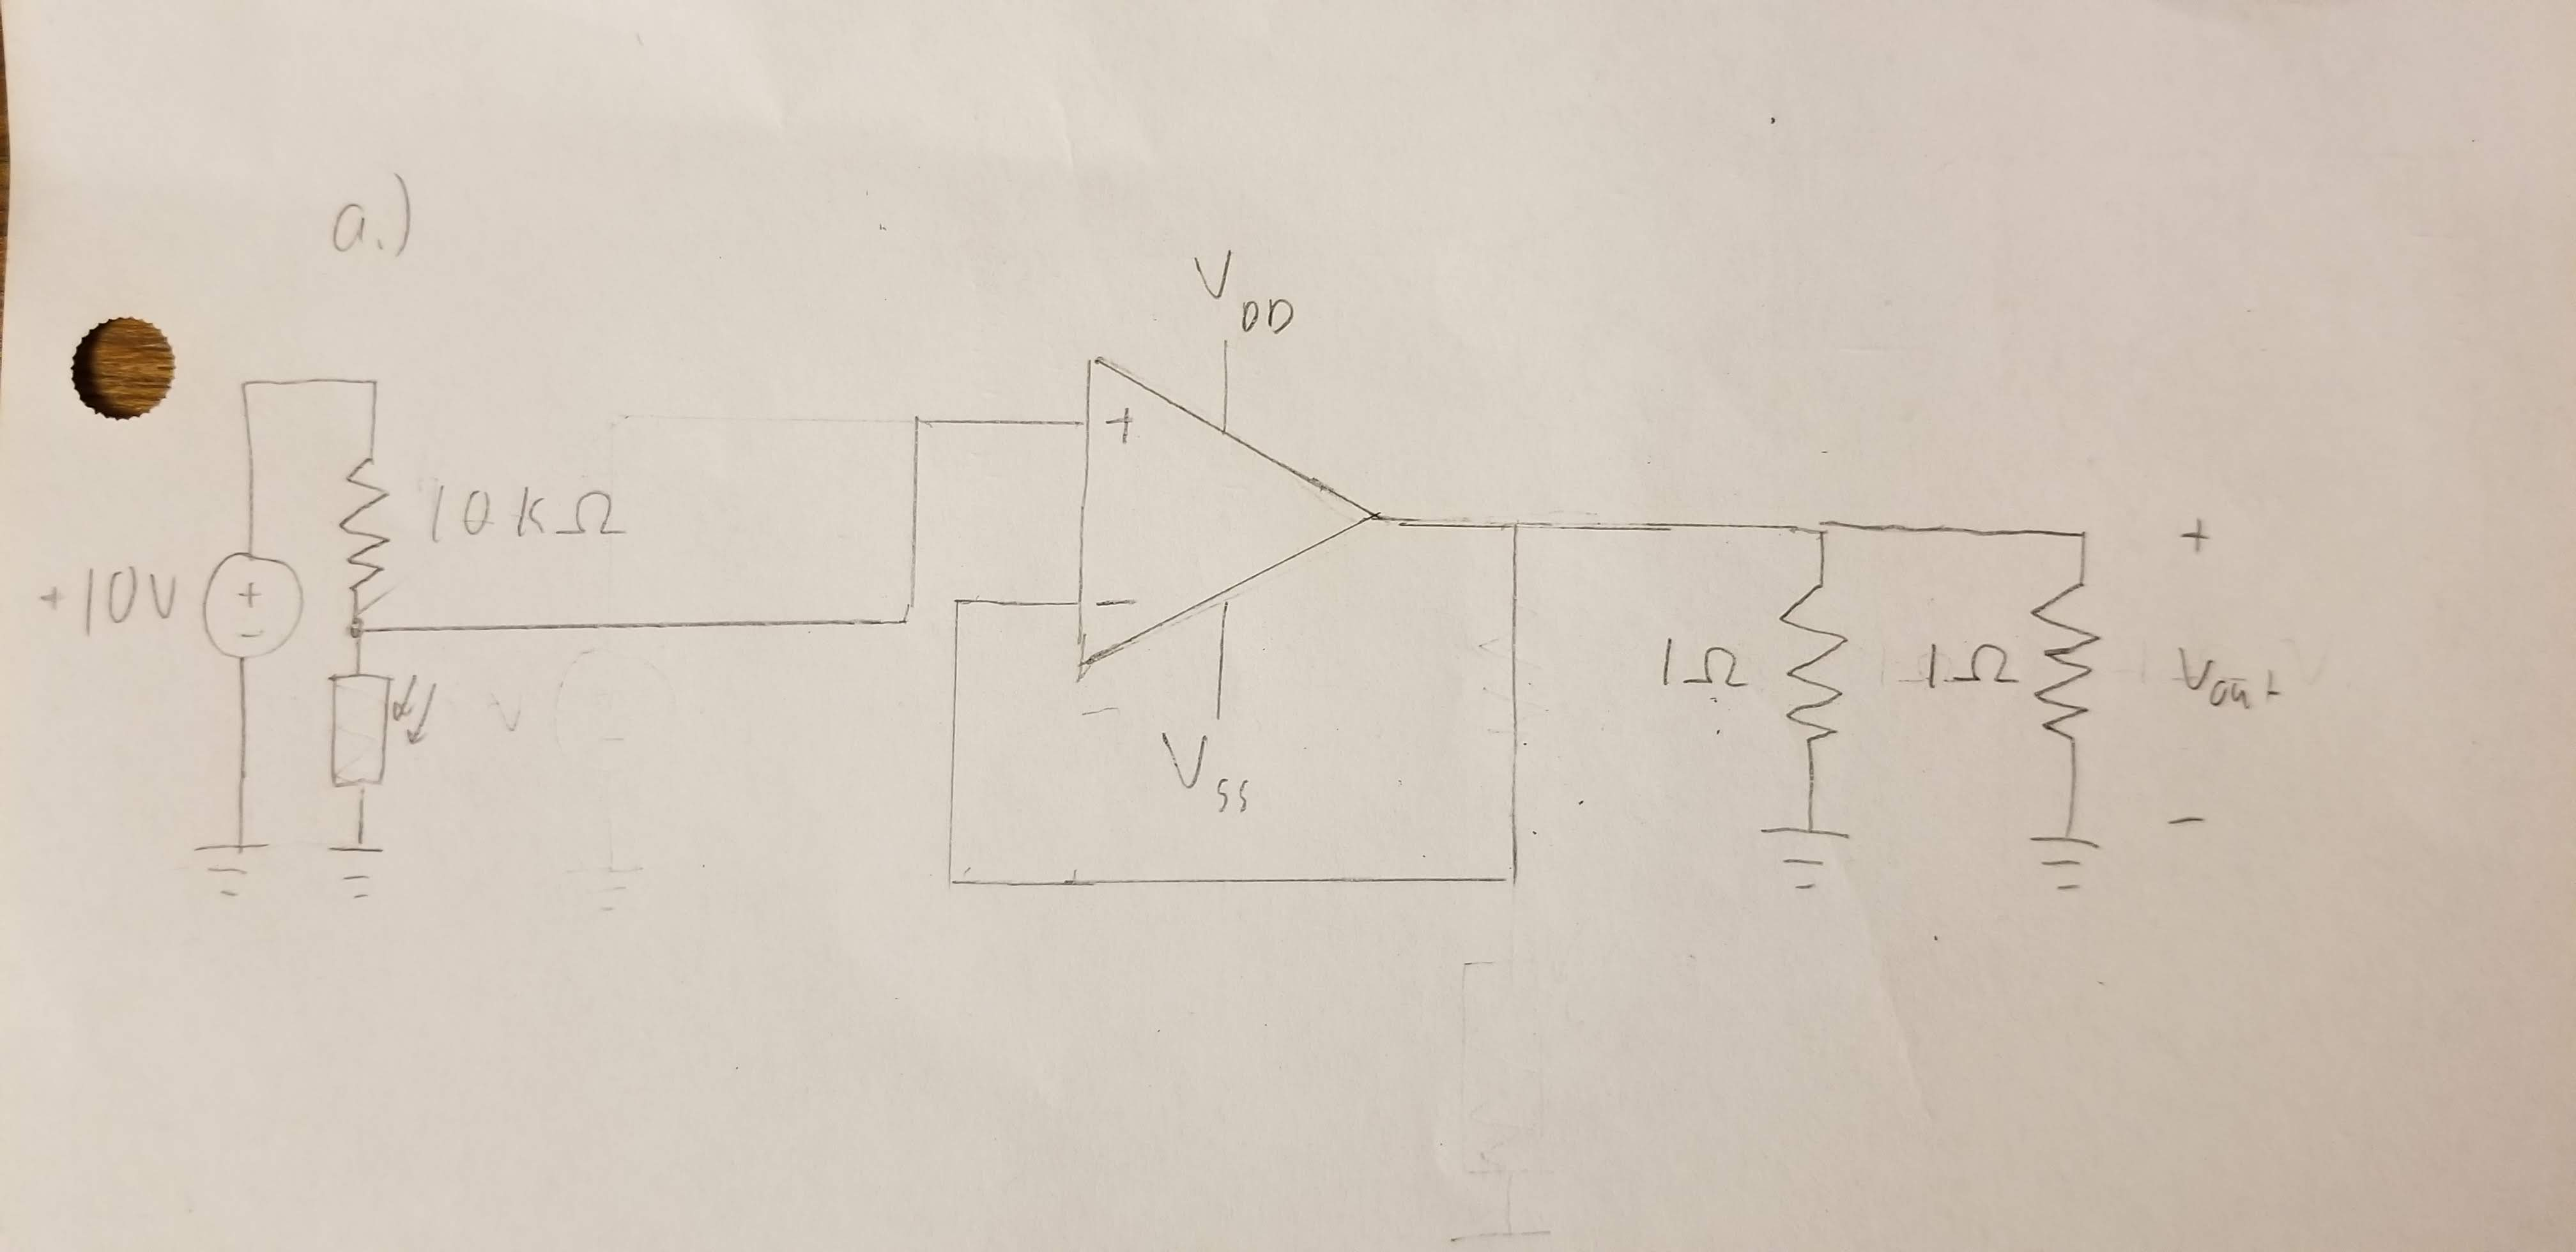
\includegraphics[width=0.7\linewidth]{20191115_175023}
\end{center}

At the front, it is clear that the voltage divider should half the voltage from the \SI{10}{\volt} source if we set the top resistor to \SI{10}{\kilo\ohm}. 
Furthermore, at the closest, the output voltage is 
\begin{equation}
	v_{in} = \SI{10}{\volt} \frac{\SI{100}{\ohm}}{\SI{10}{\kilo\ohm} + \SI{100}{\ohm}} \approx \SI{0.099}{\volt}
\end{equation}
The buffer ensures that the motor itself does not draw any current from the voltage divider, so the output voltage remains the same on both ends. 
Then, the voltage across both motors is simply \(v_{in}\), which are placed in parallel to ensure the same voltage across both. 

\subsection{Distance Control}

\begin{center}
	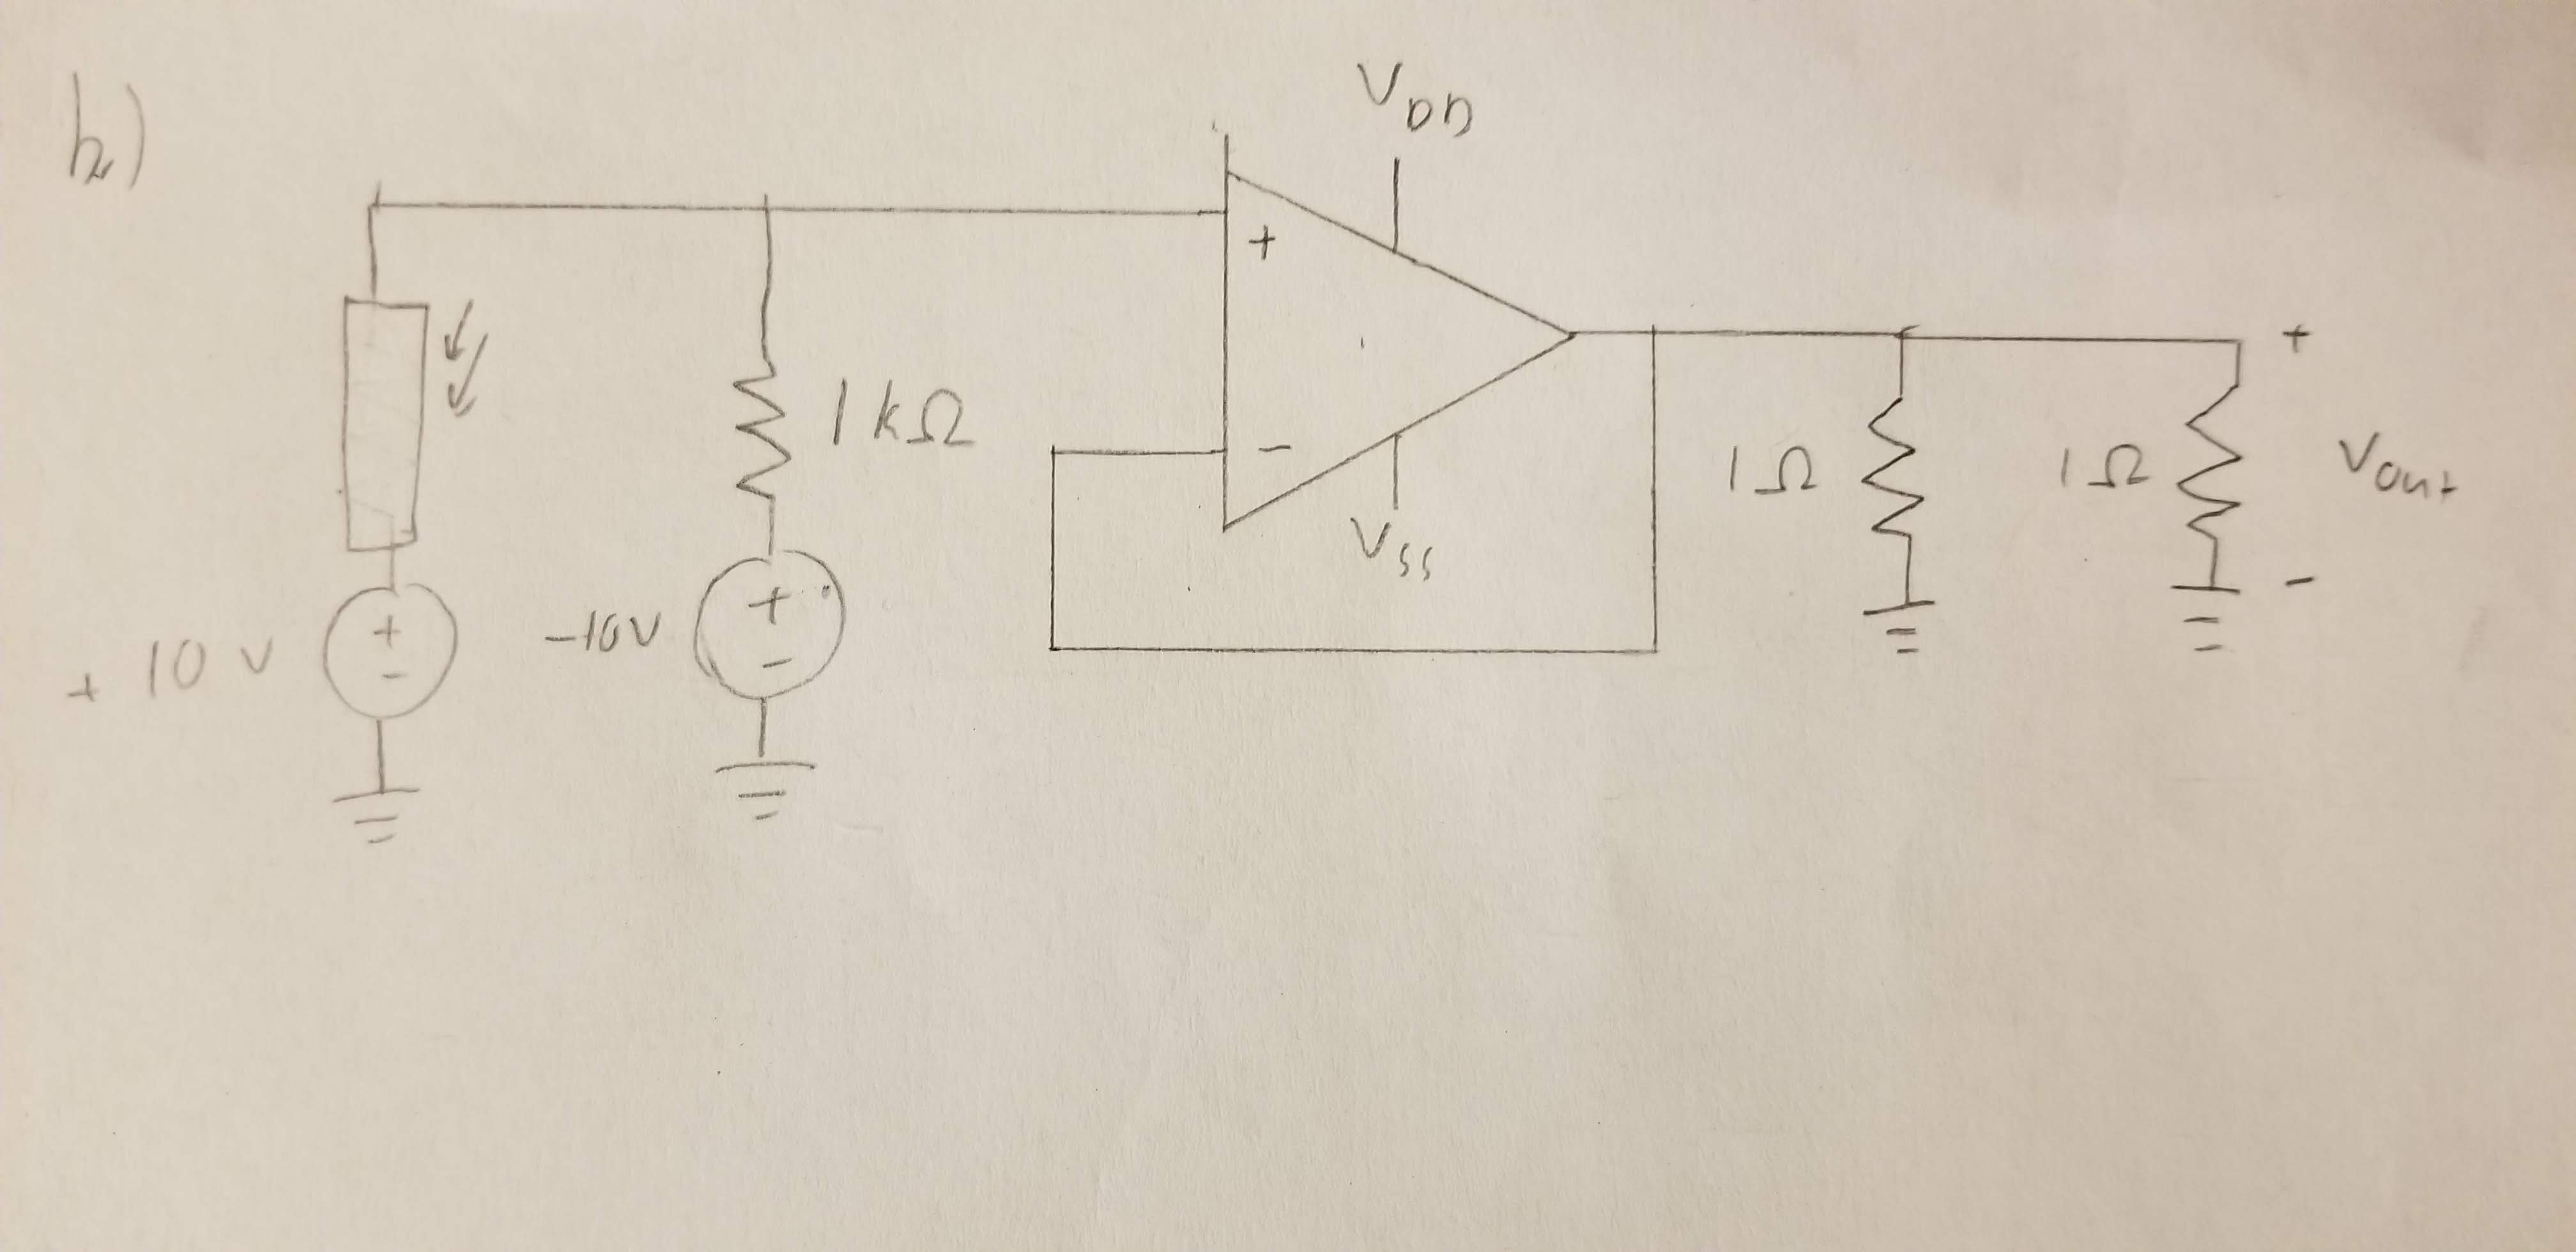
\includegraphics[width=0.7\linewidth]{20191115_175034}
\end{center}

Using the voltage summer, we can set its equation equal to zero while setting an arbitrary resistor to \SI{1}{\kilo\ohm}, 
\begin{align}
	0 &= 10 \frac{\SI{1}{\kilo\ohm}}{\SI{1}{\kilo\ohm} + R_2} - 10 \frac{R_2}{\SI{1}{\kilo\ohm} + R_2} \\
	R_2 &= \SI{1}{\kilo\ohm}
\end{align}
Some more checking ensures that when \(R_{photo} < \SI{1}{\kilo\ohm}\), \(v_{in} < \SI{0}{\volt}\), and vice versa. 
Once more, the buffer ensures no current draw from the summer, and our motors remain in the same configuration. 

\section{Op Amp Nodal Analysis}

\subsection{}

\begin{center}
	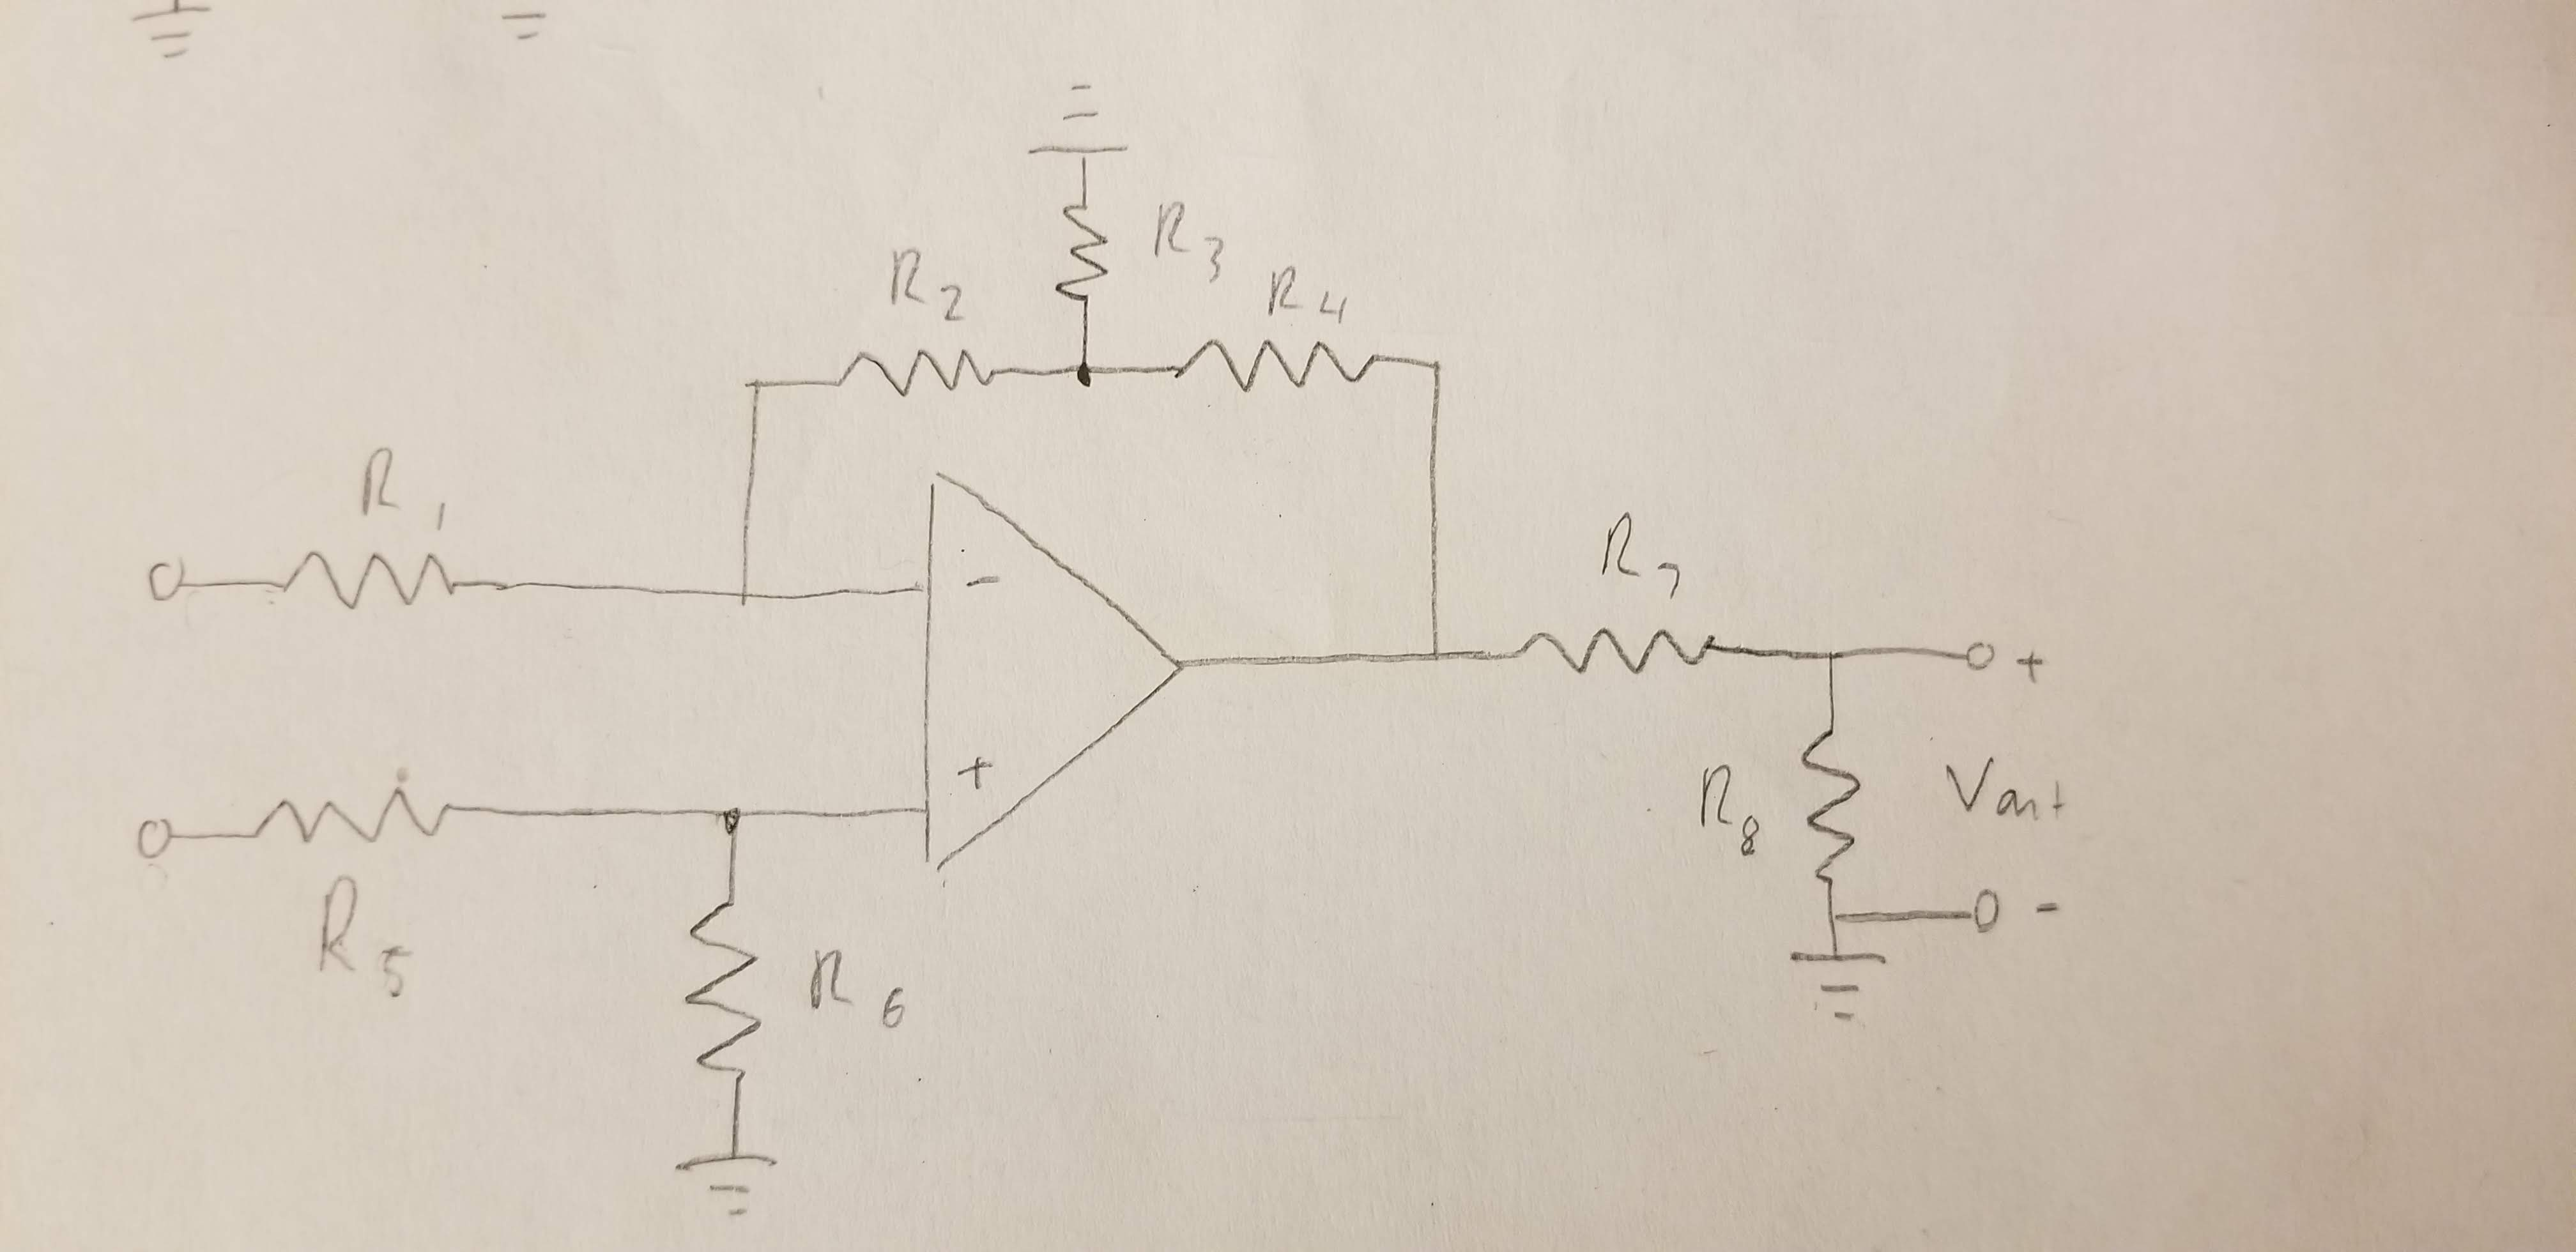
\includegraphics[width=0.7\linewidth]{20191115_175737}
\end{center}

\subsection{}

Performing KCL on the negative, positive, feedback, and output nodes gives us
\begin{align}
	I_{R_1} - I_{R_2} &= 0 \\
	I_{R_5} - I_{R_6} &= \\
	I_{R_2} - I_{R_3} - I_{R_4} &= \\
	I_{R_4} - I_{R_7} &= \\
	I_{R_7} - I_{R_8} &=
\end{align}
Substituting node voltages, 
\begin{align}
	\frac{V_1 - V^-}{R_1} - \frac{V^- - u_1}{R_2} &= 0 \\
	\frac{V_2 - V^+}{R_5} - \frac{V^+}{R_6} &= \\
	\frac{V^- - u_1}{R_2} - \frac{u_1}{R_3} - \frac{u_1 - u_2}{R_4} &= \\
	\frac{u_1 - u_2}{R_4} - \frac{u_2 - u_3}{R_7} &= \\
	\frac{u_2 - u_3}{R_7} - \frac{u_3}{R_8} &=
\end{align}
Some linear algebra yields the solution
\begin{equation}
	\begin{bmatrix}
	V^+ \\
	V^- \\
	u_1 \\
	u_2 \\
	u_3
	\end{bmatrix}
	=
	\begin{bmatrix}
	\frac{R_6 \cdot V_2}{R_5+R_6} \\
	\frac{R_2 \cdot R_3 \cdot V_1+R_2 \cdot R_4 \cdot V_1+R_3 \cdot R_4 \cdot V_1+R_2 \cdot R_7 \cdot V_1+R_3 \cdot R_7 \cdot V_1+R_2 \cdot R_8 \cdot V_1+R_3 \cdot R_8 \cdot V_1}{R_1 \cdot R_3+R_2 \cdot R_3+R_1 \cdot R_4+R_2 \cdot R_4+R_3 \cdot R_4+R_1 \cdot R_7+R_2 \cdot R_7+R_3 \cdot R_7+R_1 \cdot R_8+R_2 \cdot R_8+R_3 \cdot R_8} \\
	\frac{R_3 \cdot R_4 \cdot V_1+R_3 \cdot R_7 \cdot V_1+R_3 \cdot R_8 \cdot V_1}{R_1 \cdot R_3+R_2 \cdot R_3+R_1 \cdot R_4+R_2 \cdot R_4+R_3 \cdot R_4+R_1 \cdot R_7+R_2 \cdot R_7+R_3 \cdot R_7+R_1 \cdot R_8+R_2 \cdot R_8+R_3 \cdot R_8} \\
	\frac{R_3 \cdot R_7 \cdot V_1+R_3 \cdot R_8 \cdot V_1}{R_1 \cdot R_3+R_2 \cdot R_3+R_1 \cdot R_4+R_2 \cdot R_4+R_3 \cdot R_4+R_1 \cdot R_7+R_2 \cdot R_7+R_3 \cdot R_7+R_1 \cdot R_8+R_2 \cdot R_8+R_3 \cdot R_8} \\
	\frac{R_3 \cdot R_8 \cdot V_1}{R_1 \cdot R_3+R_2 \cdot R_3+R_1 \cdot R_4+R_2 \cdot R_4+R_3 \cdot R_4+R_1 \cdot R_7+R_2 \cdot R_7+R_3 \cdot R_7+R_1 \cdot R_8+R_2 \cdot R_8+R_3 \cdot R_8}
	\end{bmatrix}
\end{equation}
with our node of interest being \(u_3\), 
{\small
\begin{equation}
	u_3 = \frac{R_3 \cdot R_8 \cdot V_1}{R_1 \cdot R_3+R_2 \cdot R_3+R_1 \cdot R_4+R_2 \cdot R_4+R_3 \cdot R_4+R_1 \cdot R_7+R_2 \cdot R_7+R_3 \cdot R_7+R_1 \cdot R_8+R_2 \cdot R_8+R_3 \cdot R_8}
\end{equation}}

\subsection{}

Since \(V_1 = V_2 = 0\), we can connect the circuit like so:
\begin{center}
\begin{circuitikz}[american]
	\draw (0, 0) to[R=\(R_6\)] (0, 3) to[R=\(R_2\)] (0, 6);
	\draw (3, 0) to[R=\(R_3\)] (3, 6);
	\draw (6, 0) to[R=\(R_8\)] (6, 2) to[R=\(R_7\)] (6, 4) to[R=\(R_4\)] (6, 6);
	\draw (0, 0) to[short] (7, 0) node[ocirc]{\, \(a\)};
	\draw (0, 6) to[short] (6, 6);
	\draw (6, 2) to[short] (7, 2) node[ocirc]{\, \(b\)};
\end{circuitikz}
\end{center}
\begin{equation}
	R_{Th} = R_{ab} = (((R_6 + R_2) \parallel R_3) + R_4 + R_7) \parallel R_8
\end{equation}

\subsection{}

\begin{center}
\begin{circuitikz}[american]
	\draw (0, 2) to[V=\(u_3\)] (0, 0);
	\draw (0, 2) to[R=\(R_{ab}\)] (3, 2) node[ocirc]{\, \(a\)};
	\draw (0, 0) to[short] (3, 0) node[ocirc]{\, \(b\)};
\end{circuitikz}
\end{center}
See previous problems for provided values. 

\section{Homework Process and Study Group}

I did this homework by myself. 

\newpage

%\includepdf[pages=-]{prob \cdot .pdf}

\end{document}
